\chapter{信号输入输出耦合装置}
我们知道,电子注和高频电磁场是在螺旋线中交换能量的,那么高频场是怎样进入螺旋线的呢?放大后的高频场又是怎样从螺旋线中取出来的呢?原来这些工作都是由输能装置来完成的。输能装置包括信号输入和输出耦合装置,通常它们是相同的,因此下面我们统称输能装置。

\section{对输能装置有什么要求?}

最常用的微波传输线有两种形式,即波导和同轴线,因此输能装置实际上就是管内的螺旋线和管外的波导或同轴线之间的一个转换装置。对于输能装置有下面几点要求:

\begin{enumerate}
	\item 损耗小。例如:对输出端来说,我们希望放大了的信号经过输能装置后,能尽量作到接近100\%地经波导或同轴线传输给负载,成为有用的信号。同样,在输入端希望外界提供的信号能全部进入螺旋线。然而,由于输能装置总有一定损耗,因此信号经过时必有一定衰减。我们只能设法降低输能装置的损耗,使信号的损失尽可能少些。
	\item 匹配好。大家知道,每一种传输线(如波导、同轴线)都有它的特性阻抗,当两个特性阻抗不一样的传输线接在一起时,信号传输到连接处就要遇到反射。两者特性阻抗相差多,反射也就越大,通常我们称这种情况为阻抗不匹配。常用的同轴线是50欧姆的,而螺旋线的阻抗为几十到一百多欧姆,两者是不相等的,因此就要求输能装置能够起阻抗变换的作用,把两个阻抗匹配起来,这样,当信号通过输能装置时,反射就小,损失也就小。
	\item 频带宽。在中小功率行波管中我们几乎都采用色散特性良好的螺旋线作为慢波系统,因此行波管的频带应是很宽的。由于行波管的信号必须通过输能装置才能进入螺旋线,而输能装置的频带通常要比螺旋线窄,因此行波管的频带常常受限于输能装置。往往是输能装置的频带宽度决定了行波管的频带宽度,可见,尽量把输能装置的频带做得宽些是有重要意义的。
	\item 体积小。行波管的输能装置周围,有行波管必不可少的部分一磁聚束系统。由于输能装置必须占有一定的空间,因此就必然会影响磁聚束系统对电子注的聚束。我们希望输能装置的体积要尽可能小。这样,对聚束的影响就小,使用起来也方便。
	\item 结构简单、容易调节。
\end{enumerate}
\section{输能装置有哪几种?}
通常,能够基本上实现上述要求的输能装置有直接引出型、同轴腔耦合型、反绕螺旋线型和波导耦合型等几种型式。
\subsection{直接引出型}
图\ref{ch9-1}是一种直接引出型的输能装置的结构。螺旋线两端是分别通过筒形密封陶瓷窗侧壁的金属封接小针与管外同轴线的内导体相连接的,因此称为筒形窗直接引出型耦合装置。同轴线的外导体则和金属管壳相连。由于管外同轴线的阻抗是50欧姆,而螺旋线的特性阻抗一般要比50欧姆大,因此为了保证良好的匹配,通常要把螺旋线拉直一段,然后再和陶瓷窗侧壁封接的金属小针焊接,同时还要在管外的同轴插座内设计一些过渡的零件,使得螺旋线和同轴线能够很好地匹配。
\begin{figure}[phtb]
	\centering
	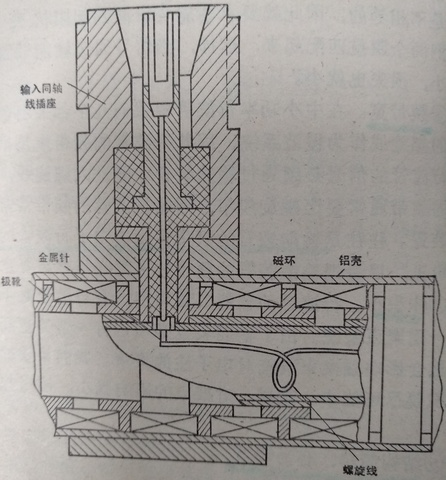
\includegraphics[width=0.75\linewidth]{figure/ch9-1}
	\caption{ 筒形窗直接引出型耦合装置}
	\label{ch9-1}
\end{figure}

图\ref{ch9-2}是另一种直接引出型耦合装置的结构示意图,这种耦合装置的陶瓷窗是锥形窗。和筒形窗相比,锥形窗耦合装置有下面两个优点:(1)结构紧凑,高频泄漏小,因此更适宜于用在频率较高的管子中(如三厘米以上的波段)。筒形窗结构耦合装置在高频时泄漏大,因而要影响到整管的增益特性,甚至引起自激振荡。(2)锥形窗的耦合装置的驻波比可以做得比筒形窗更小些,一般在1.5以下,而筒形窗耦合装置的驻波比一般只能在2以下。锥形窗耦合装置的频带也比筒形窗要宽,例如:采用锥形窗耦合装置的某行波管,其工作频率范围为2-12千兆赫。筒形窗耦合装置的频带也比较宽,例如采用筒形窗耦合装置的某两种行波管,它们的工作频率范围分别为2-4干兆赫和4-8千兆赫。它们的插入损耗都比较小(小于0.5分贝)但是,锥形窗的制造工艺要比筒形窗复杂,这是它的缺点。
\begin{figure}[phtb]
	\centering
	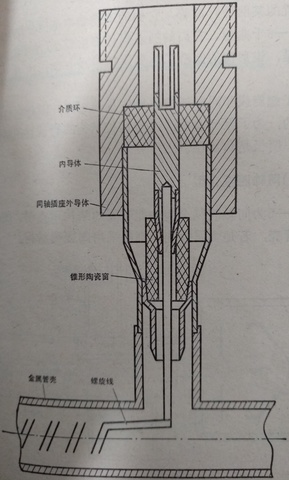
\includegraphics[width=0.7\linewidth]{figure/ch9-2}
	\caption{ 锥形窗直接引出型耦合装置}
	\label{ch9-2}
\end{figure}

由于螺旋线和同轴线的内导体直接相连,因此它们之间是等电位的,为了保证安全,通常这种结构的行波管的螺旋线是接地的,阴极是负高压。

\subsection{同轴腔耦合型}
图\ref{ch9-3}为同轴腔耦合型输能装置的结构示意图。图中画的是玻璃管壳,若是金属管壳,则需采用陶瓷窗结构。
\begin{figure}[phtb]
	\centering
	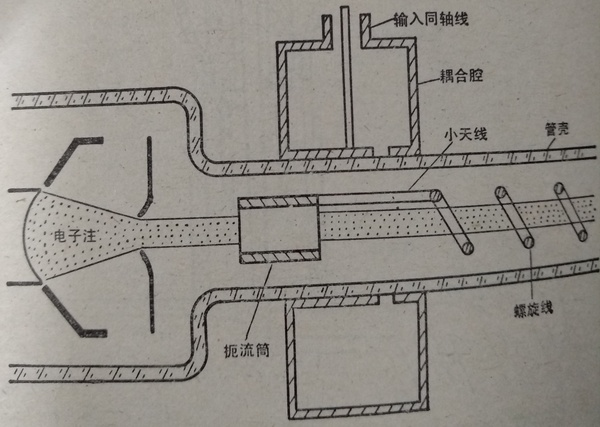
\includegraphics[width=0.75\linewidth]{figure/ch9-3}
	\caption{ 同轴腔耦合结构示意图}
	\label{ch9-3}
\end{figure}

高频信号由同轴线输入,在腔体内激励起电磁场,然后耦合到螺旋线的天线上去。这种装置的优点是陶瓷窗的侧壁不需要开孔和金属小针封接,因为信号是通过插在同轴腔中的螺旋线天线耦合而不是通过金属小针耦合的。因此陶瓷窗的工艺可以大为简化。不过,这种耦合装置的频带较窄,体积较大,很难用于周期场聚束系统,因此很少被采用。

\subsection{反绕螺旋线型}
图\ref{ch9-4}为反绕螺旋线型输能装置示意图。它是在玻璃管壳外与管内螺旋线同心地反绕一段螺旋线构成的。设计反绕螺旋线的尺寸时应当使内外螺旋线中电磁场的相速度相等,外螺旋线的一端接以50欧姆负载,另一端接同轴线的内导体。这样,高频能量就能从内螺旋线传到外螺旋线上去,然后再由连接外螺旋线的同轴线传输出去。反绕螺旋线耦合装置的理论分析从略。
\begin{figure}[phtb]
	\centering
	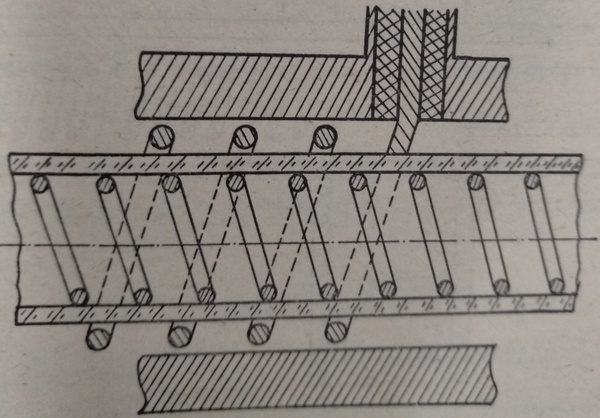
\includegraphics[width=0.75\linewidth]{figure/ch9-4}
	\caption{ 反绕螺旋线型输能装置示意图}
	\label{ch9-4}
\end{figure}

采用反绕螺旋线耦合也可以得到很宽的频带,结构和工艺都较简单,且体积较小,因此可用于周期场聚束系统中。另外,它的耦合位置也可以在管壳外任意调节,这是它的优点。它的缺点是损耗较大,约在0.5-1分贝,且功率大于1千瓦时容易打火。目前,在玻璃结构的行波管中仍有用此结构的,但在金属陶瓷结构的行波管中,因反而要带来一些麻烦(要求陶瓷窗的长度增加)损耗又大,故不采用。
\subsection{波导耦合型}
前面所讲的三种耦合装置都是转换至同轴线系统的输能装置,这里要讲的是转换至波导系统的输能装置,它的结构如图\ref{ch9-5}所示。
\begin{figure}[phtb]
	\centering
	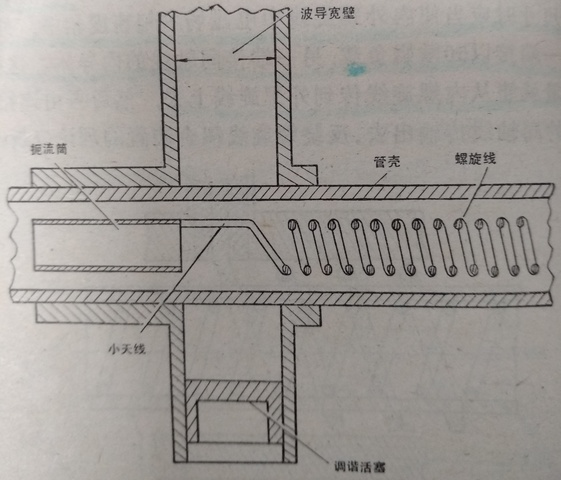
\includegraphics[width=0.75\linewidth]{figure/ch9-5}
	\caption{ 波导耦合型输能装置示意图}
	\label{ch9-5}
\end{figure}


取一段波导在其宽壁中间打一个比行波管管壳稍粗的孔行波管穿过此孔放入其中,管内螺旋线两端拉直,构成输入端和输出端的两个小天线,为了防止高频场沿轴线跑出去,在小天线终端需要焊一个扼流筒。小天线的位置正好落在波导窄壁中间,因此就能利用小天线将能量从螺旋线传输到波导系统中去。由于波导占有一定的空间,其内没有磁钢,因此波导内磁场将减弱,对聚束会带来影响。于是我们常把波导的高度减小,做成所谓“减高波导”,这样就可以尽量少占有一些聚束系统的空间,以减小对聚束的影响。那么减高波导又怎样和外面的标准波导相连接呢?通常用阻抗变换器来完成这个任务,它们可以是阶梯变换器,也可以是渐变形的变换器。为了调节匹配,还需在波导的另一端装上短路活塞。


波导耦合装置的优点是:高频损耗小,匹配好。这对于改善整管的增益特性是有利的,因此是一个很大的优点。此外管子本身的工艺和结构也比较简单。


波导耦合装置的缺点是:周期聚束系统中使用比较困难因为波导本身有一定的尺寸(即使减小了高度,仍有较大的尺寸),又不能将磁环放进波导中去,因此,在波导插入的地方行波管轴上的磁场就要跌落,破坏了磁场的均匀性。为克服磁场跌落,常常要在减高波导的两边附加强磁场,作为补偿措施,但是这样就使耦合装置的频带较窄,一般只能做到中心频率的40\%。


上面,我们对几种输能装置作了简单的介绍。行波管输能装置对于其高频性能有很大的影响。由于影响输能装置性能的因素很多(管内管外不少零件的尺寸、位置都有影响),因此,常常需要经过许多次反复试验才能得到一种性能良好的输能装置。
